\documentclass[12pt, a4paper]{report}
\usepackage{hyperref}
\usepackage[top=3cm,right=3cm,bottom=3cm,left=2.5cm]{geometry}
\usepackage{caption}
\usepackage{indentfirst}
\usepackage{graphicx}
\usepackage{subfigure}
\usepackage{float}
\usepackage{fancyhdr}
\usepackage{titlesec}
\usepackage{tikz}
\setcounter{secnumdepth}{4}
\setcounter{tocdepth}{4}


\pagestyle{fancy}
% Set up fancyhdr to place page number at the top left
\pagestyle{fancy}
\fancyhf{} % Clear all header/footer fields
\fancyhead[L]{\thepage} % Page number on the top left

% Define custom style for chapter page (no header or footer)
\fancypagestyle{plain}{
	\fancyhf{} % Clear headers and footers
	\renewcommand{\headrulewidth}{0pt} % Remove header rule
}


% Changing TOC addressing format (from period separation to dash seperation)
\renewcommand{\thesection}{\thechapter-\arabic{section}-}
\renewcommand{\thesubsection}{\thechapter-\arabic{section}-\arabic{subsection}-}
\renewcommand{\thesubsubsection}{\thechapter-\arabic{section}-\arabic{subsection}-\arabic{subsubsection}-}

\renewcommand{\thetable}{(\thechapter-\arabic{table})}

% Redefine how captions are written 
\renewcommand{\thefigure}{(\thechapter-\arabic{figure})}

% Set caption font size to 11pt
\captionsetup{font=small, labelsep=space} % 'small' is equivalent to 11pt in most classes

% Automatically switch between Persian and Latin fonts based on character type
\XeTeXinterchartokenstate=1
\newXeTeXintercharclass\persianchars
\newXeTeXintercharclass\latinchars

% Automatically switch fonts when switching between Persian and Latin characters
\XeTeXinterchartoks \latinchars \persianchars = {\begingroup\persianfont\endgroup}
\XeTeXinterchartoks \persianchars \latinchars = {\begingroup\latinfont\endgroup}



\title{Trust Compiler Report}
\author{InFluX}

\begin{document}
%\maketitle
\begin{titlepage}
	\centering
	% University logo
	
\includegraphics[width=0.15\textwidth]{images/logo.png}
	
	% University and Faculty name
	{\Large Isfahan University}\par
	{\Large Computer Engineering Department}\par\vspace{2cm}
	
	% Report title
	\textbf
	{\Huge Trust Compiler Report}\par\vspace{1.5cm}
	
	% Intern details
	\large
	\textbf{Students:}\par{Zahra Masoumi - Matin Azami}\par\vspace{0.5cm}  
	\textbf{Students ID:}\par{4003623003 - 4003623003}\par\vspace{0.5cm}
	\textbf{Professor:}\par{Dr. Shafiee}\par\vspace{0.5cm}
		
	\par\vspace{2cm}
	
	
\end{titlepage}

\tableofcontents

\listoftables

\listoffigures


\chapter{Lexical Analyzer}

\section{Introduction}

\section{White Spaces}


\begin{center}
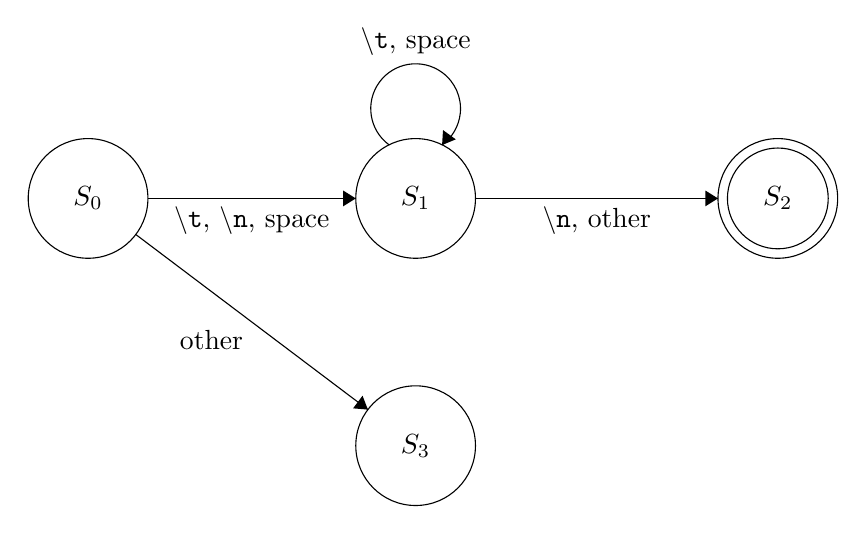
\begin{tikzpicture}[scale=0.2]
\tikzstyle{every node}+=[inner sep=0pt]
\draw [black] (4,-10.9) circle (3.8);
\draw (4,-10.9) node {$S_0$};
\draw [black] (24.8,-10.9) circle (3.8);
\draw (24.8,-10.9) node {$S_1$};
\draw [black] (47.8,-10.9) circle (3.8);
\draw (47.8,-10.9) node {$S_2$};
\draw [black] (47.8,-10.9) circle (3.2);
\draw [black] (24.8,-26.6) circle (3.8);
\draw (24.8,-26.6) node {$S_3$};
\draw [black] (7.8,-10.9) -- (21,-10.9);
\fill [black] (21,-10.9) -- (20.2,-10.4) -- (20.2,-11.4);
\draw (14.4,-11.4) node [below] {\texttt{\textbackslash t},\ \texttt{\textbackslash n},\ space};
\draw [black] (28.6,-10.9) -- (44,-10.9);
\fill [black] (44,-10.9) -- (43.2,-10.4) -- (43.2,-11.4);
\draw (36.3,-11.4) node [below] {\texttt{\textbackslash n},\ other};
\draw [black] (23.125,-7.506) arc (234:-54:2.85);
\draw (24.8,-1.85) node [above] {\texttt{\textbackslash t},\ space};
\fill [black] (26.48,-7.51) -- (27.35,-7.15) -- (26.54,-6.56);
\draw [black] (7.03,-13.19) -- (21.77,-24.31);
\fill [black] (21.77,-24.31) -- (21.43,-23.43) -- (20.83,-24.23);
\draw (11.84,-19.25) node [below] {other};
\end{tikzpicture}
\end{center}


\section{Comments}

\begin{center}
\begin{tikzpicture}[scale=0.2]
\tikzstyle{every node}+=[inner sep=0pt]
\draw [black] (4,-10.9) circle (3.8);
\draw (4,-10.9) node {$S_0$};
\draw [black] (19.9,-10.9) circle (3.8);
\draw (19.9,-10.9) node {$S_1$};
\draw [black] (35.8,-10.9) circle (3.8);
\draw (35.8,-10.9) node {$S_2$};
\draw [black] (51.2,-10.9) circle (3.8);
\draw (51.2,-10.9) node {$S_3$};
\draw [black] (19.9,-26.3) circle (3.8);
\draw (19.9,-26.3) node {$S_4$};
\draw [black] (7.8,-10.9) -- (16.1,-10.9);
\fill [black] (16.1,-10.9) -- (15.3,-10.4) -- (15.3,-11.4);
\draw (11.95,-11.4) node [below] {$/$};
\draw [black] (23.7,-10.9) -- (32,-10.9);
\fill [black] (32,-10.9) -- (31.2,-10.4) -- (31.2,-11.4);
\draw (27.85,-11.4) node [below] {$/$};
\draw [black] (39.6,-10.9) -- (47.4,-10.9);
\fill [black] (47.4,-10.9) -- (46.6,-10.4) -- (46.6,-11.4);
\draw (43.5,-11.4) node [below] {\texttt{\textbackslash n}};
\draw [black] (6.73,-13.54) -- (17.17,-23.66);
\fill [black] (17.17,-23.66) -- (16.94,-22.74) -- (16.25,-23.46);
\draw (9.38,-19.08) node [below] {$other$};
\draw [black] (19.9,-14.7) -- (19.9,-22.5);
\fill [black] (19.9,-22.5) -- (20.4,-21.7) -- (19.4,-21.7);
\draw (19.4,-18.6) node [left] {$other$};
\draw [black] (34.125,-7.506) arc (234:-54:2.85);
\draw (35.8,-1.85) node [above] {$other,\mbox{ }/$};
\fill [black] (37.48,-7.51) -- (38.35,-7.15) -- (37.54,-6.56);
\end{tikzpicture}
\end{center}


\section{Operators}

\subsection{Arithmetic Operations}

\subsection{Punctuation Marks}

\section{Numeric Values}

\subsection{HexaDecimal}

\subsection{Decimal}

\section{Keywords}

\section{Strings}

\begin{center}
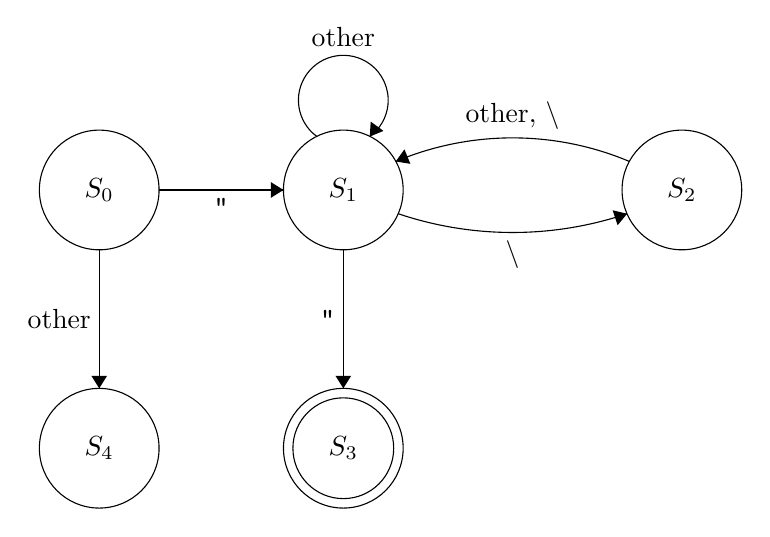
\begin{tikzpicture}[scale=0.2]
\tikzstyle{every node}+=[inner sep=0pt]
\draw [black] (4.7,-10.9) circle (3.8);
\draw (4.7,-10.9) node {$S_0$};
\draw [black] (20.2,-10.9) circle (3.8);
\draw (20.2,-10.9) node {$S_1$};
\draw [black] (41.7,-10.9) circle (3.8);
\draw (41.7,-10.9) node {$S_2$};
\draw [black] (20.2,-27.3) circle (3.8);
\draw (20.2,-27.3) node {$S_3$};
\draw [black] (20.2,-27.3) circle (3.2);
\draw [black] (4.7,-27.3) circle (3.8);
\draw (4.7,-27.3) node {$S_4$};
\draw [black] (8.5,-10.9) -- (16.4,-10.9);
\fill [black] (16.4,-10.9) -- (15.6,-10.4) -- (15.6,-11.4);
\draw (12.45,-11.4) node [below] {\texttt{"}};
\draw [black] (4.7,-14.7) -- (4.7,-23.5);
\fill [black] (4.7,-23.5) -- (5.2,-22.7) -- (4.2,-22.7);
\draw (4.2,-19.1) node [left] {other};
\draw [black] (18.525,-7.506) arc (234:-54:2.85);
\draw (20.2,-1.85) node [above] {other};
\fill [black] (21.88,-7.51) -- (22.75,-7.15) -- (21.94,-6.56);
\draw [black] (38.217,-12.408) arc (-71.36814:-108.63186:22.746);
\fill [black] (38.22,-12.41) -- (37.3,-12.19) -- (37.62,-13.14);
\draw (30.95,-14.1) node [below] {\texttt{\textbackslash}};
\draw [black] (20.2,-14.7) -- (20.2,-23.5);
\fill [black] (20.2,-23.5) -- (20.7,-22.7) -- (19.7,-22.7);
\draw (19.7,-19.1) node [left] {\texttt{"}};
\draw [black] (23.533,-9.089) arc (112.82624:67.17376:19.118);
\fill [black] (23.53,-9.09) -- (24.46,-9.24) -- (24.08,-8.32);
\draw (30.95,-7.09) node [above] {other, \texttt{\textbackslash}};
\end{tikzpicture}
\end{center}


\section{IDs}


\end{document}